%macbook
\setcounter{paragraph}{0}
\PhanI
\loai{Thay số tính bước sóng}
\begin{ex}%[3P2Y1-2][Loai1] 
Một sóng cơ lan truyền đi với vận tốc 2 m/s với tần số 50 Hz. Bước sóng của sóng này có giá trị là
\choice
{1 cm}
{0,04 cm}
{100 cm}
{\True 4 cm}
\loigiai{
Bước sóng của sóng trên: $\lambda =\dfrac{v}{f} =\dfrac{2}{50} = 0,04\ m = 4\ cm$.\\
}
\end{ex} \haidong{20}


\loai{Quãng đường lan truyền của sóng}
\begin{ex}%[3P2K1-2][Loai1] 
Một sóng cơ có bước sóng là 12 cm. Trong 3,5 chu kì dao động của một phần tử sóng, sóng truyền được quãng đường là
\choice
{\True 42 cm}
{21 cm}
{3,43 cm}
{51,2 cm}
\loigiai{
%\begin{itemize}
%\item 
Trong 1 T sóng truyền được quãng đường $\lambda$.
%\item 
$\Rightarrow$ 3,5T sóng truyền được quãng đường $S = 3,5\lambda = 3,5.12 = 42$ cm.
%\end{itemize}
}
\end{ex} \haidong{20}
\begin{ex}%[3P2K1-2][Loai1] 
Người ta gây ra một dao động ở đầu O một dây cao su căng thẳng, tạo nên một dao động theo phương vuông góc với vị trí bình thường của dây, với biên độ 3 cm và chu kì 1,8 s. Sau 3 s chuyển động truyền được 15 m dọc theo dây. Bước sóng của sóng tạo thành trên dây là
\choice
{\True 9,0 m}
{4,5 m}
{3,2 m}
{6,4 m}
\loigiai{
Ta có: $v_s=\dfrac{15}{3}=5\ m\Rightarrow \lambda=v_s.T=5.1,8=9\ m$. \\
Ta có: $v_s = \dfrac{15}{3} = 5\ m\Rightarrow \lambda = v_s.T = 5.1,8 = 9\ m$.
}
\end{ex} \haidong{20}
\begin{ex}%[3P2Y1-2][Loai1] 
Sóng cơ truyền trên một sợi dây rất dài với khoảng cách giữa hai đỉnh sóng kế tiếp là 20 cm. Bước sóng $\lambda $ có giá trị bằng
\choice
{10 cm}
{\True 20 cm}
{5 cm}
{40 cm}
\loigiai{
Khoảng cách giữa hai đỉnh sóng liên tiếp chính bằng một bước sóng nên: $\lambda =20\ cm$.
}
\end{ex} \haidong{20}
%\loai{Quan sát phao nhô lên}


\begin{ex}%[3P2B1-2][Loai1] 
Một người quan sát thấy một cánh hoa trên hồ nước nhô lên 10 lần trong khoảng thời gian 36 s. Khoảng cách giữa ba đỉnh sóng kế tiếp là 24 m. Tốc độ truyền sóng trên mặt hồ là
\choice
{\True 3 m/s}
{3,32 m/s}
{3,76 m/s}
{6,0 m/s}
\loigiai{
Ta có: $\begin{cases}
T=\dfrac{\Delta t}{n-1}=\dfrac{36}{10-1}=4\ s\\
\lambda =\dfrac{\Delta x}{m-1}=12\ m\\
\end{cases}\Rightarrow v=\dfrac{\lambda}{T}=3\ m/s$}

\end{ex} \haidong{20}

 
\begin{ex}%KNTT
\immini[thm]{Trong thí nghiệm ở hình dưới đây, cần rung với tần số 50 Hz. Người ta đo được bán kính của 2 gợn sóng hình tròn liên tiếp lần lượt bằng: 12,4 cm và 14,3 cm. Tốc độ truyền sóng là
\motcot
{\True 95 cm/s}
{105 cm/s}
{75 cm/s}
{80 cm/s}
}
{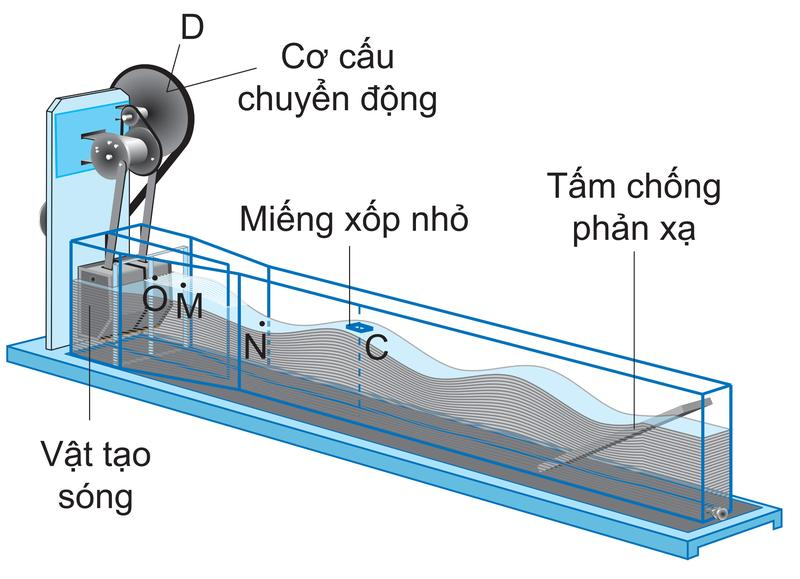
\includegraphics[width=7cm]{Hinh/KN81}}
\loigiai{
%\begin{itemize}
%\item 
Bước sóng là khoảng cách giữa hai gợn sóng liên tiếp, theo đề bài ta có: $\lambda=14,3-12,4=1,90\ cm$.\\
%\item 
Áp dụng công thức: $v=\lambda f=1,9.50=95\ cm/s$.
%\end{itemize}
}
\end{ex} \haidong{20}

%\loai{Quãng đường truyền sóng - quãng đường dao động}
\begin{ex}%[3P2K1-2][Loai1] 
Một sóng cơ lan truyền trong một môi trường với tốc độ 1 m/s và tần số 10 Hz, biên độ sóng 4 cm. Khi phần tử vật chất của môi trường đi được quãng đường 8 cm thì sóng truyền được quãng đường
\choice
{4 cm}
{10 cm}
{8 cm}
{\True 5 cm}
\loigiai{
\begin{itemize}
\item Phần tử vật chất di chuyển được quãng đường $8 \ cm = 2a$ tức là dao động trong thời gian $\dfrac{T}{2}$.
\item Trong 1 T sóng truyền được quãng đường $\lambda\Rightarrow \dfrac{T}{2}$ sóng truyền được quãng đường $S = \dfrac{\lambda }{2} = \dfrac{v}{2f} = \dfrac{1}{2.10} = 0,05 = 5$ cm. 
\end{itemize}
}
\end{ex} \haidong{20}
%\loai{Lập tỉ lệ}
\begin{ex}%[3P2B1-2][Loai1]
Sóng truyền trong một môi trường đàn hồi với tốc độ truyền sóng 360 m/s. Ban đầu tần số sóng là 180 Hz. Để có bước sóng là 0,5 m thì cần tăng hay giảm tần số sóng một lượng như nào?
\choice
{Tăng thêm 420 Hz}
{\True Tăng thêm 540 Hz}
{Giảm bớt 420 Hz}
{Giảm xuống còn 90 Hz}
\loigiai{
Tần số sóng $f=\dfrac{v}{\lambda }=720\ Hz \Rightarrow$ tần số tăng một lượng $720 -180 = 540$ Hz.\\
}
\end{ex} \haidong{20}
%\loai{Hai sóng}
















%macbook 
\begin{ex}
Dải tần số mà một học sinh có thể nghe thấy từ 30 Hz đến 16000 Hz. Tốc độ truyền âm trong không khí là 330 m/s. Bước sóng ngắn nhất của âm thanh trong không khí mà bạn học sinh đó nghe được là
\choice
{\True 0,02 m}
{0,03 m}
{0,04 m}
{0,05 m}
\loigiai{
\begin{itemize}
\item Dải tần số mà học sinh có thể nghe thấy từ 30 Hz đến 16000 Hz 
\item Nên bước sóng ngắn nhất của âm thanh trong không khí mà bạn học sinh đó nghe được ở tần số 16000 Hz.
\item $\lambda=\dfrac{v}{f}=\dfrac{330}{16000}\approx 0,02\ m$. 
\end{itemize}
}
\end{ex} \haidong{20}
\loai{Sóng âm truyền trong các môi trường}
\begin{ex}%[3P2BB-2][Loai1]
Sóng âm truyền từ nước ra ngoài không khí. Tốc độ truyền sóng trong các môi trường nước và không khí lần lượt là 1480 m/s và 340 m/s. Cho biết bước sóng khi truyền trong nước là 0,74 m. Bước sóng khi ra ngoài không khí xấp xỉ bằng
\choice
{1,61 m}
{0,54 m}
{\True 0,17 m}
{85 mm}
\loigiai{
\begin{itemize}
\item Khi truyền từ môi trường nước sang môi trường không khí thì tần số sóng không thay đổi.
\item Ta có: $f = \dfrac{v_n}{\lambda_n} = \dfrac{v_{kk}}{\lambda_{kk}}$
$\Rightarrow \lambda_{kk} = \dfrac{v_{kk}}{v_n}.\lambda_n = \dfrac{340}{1480}.0,74 = 0,17\ m$. 
\end{itemize}
}
\end{ex} \haidong{20}
\begin{ex}%[3P2BB-2][Loai1]
Với máy dò dùng siêu âm, chỉ có thể phát hiện được các vật có kích thước cỡ bước sóng của siêu âm. Siêu âm trong một máy dò có tần số xác định. Trong không khí, máy dò này phát hiện được những vật có kích thước cỡ 0,068 mm. Biết vận tốc truyền âm trong không khí và trong nước lần lượt là 340 m/s và 1500 m/s. Trong nước máy dò này phát hiện được những vật có kích thước cỡ
\choice
{\True 0,3 mm}
{0,15 mm}
{0,6 mm}
{0,1 mm}
\loigiai{
\begin{itemize}
\item Do tần số của siêu âm có tần số xác định nên chu kì của nó không thay đổi khi truyền qua các môi trường.
\item Mà $\lambda_{kk} = v_{kk}.T$; $\lambda_{n} = v_n.T\Rightarrow \dfrac{\lambda_{kk}}{v_{kk}} = \dfrac{\lambda_n}{v_n} \Rightarrow \lambda_n = \lambda_{kk}\dfrac{v_n}{v_{kk}} = 0,068.\dfrac{1500}{340} = 0,3\ mm$.
\end{itemize}
}
\end{ex} \haidong{20}

\loai{Sự truyền âm}
\begin{ex}%[3P2BB-2][Loai1]
Một người đứng gần ở chân núi hú lên một tiếng. Sau 8 s thì nghe tiếng mình vọng lại, biết tốc độ âm trong không khí là 340 m/s. Khoảng cách từ chân núi đến người đó là
\choice
{1333 m}
{1386 m}
{\True 1360 m}
{1320 m}
\loigiai{
\begin{itemize}
\item Thời gian sóng âm cả đi và về phải thỏa mãn: $t=\dfrac{2L}{v}\Rightarrow L=1360\ m$. 
\end{itemize}
}
\end{ex} \haidong{20}


\begin{ex}%[3P2KB-2][Loai1]
Một người dùng búa gõ vào đầu một thanh nhôm. Người thứ hai ở đầu kia áp tai vào thanh nhôm và nghe được âm của tiếng gõ hai lần (một lần qua không khí, một lần qua thanh nhôm). Khoảng thời gian giữa hai lần nghe được là 0,12 s. Biết vận tốc truyền âm trong không khí là 330 m/s, trong nhôm là 6420 m/s. Chiều dài của thanh nhôm là
\choice
{34,25 m}
{4,17 m}
{342,5 m}
{\True 41,7 m}
\loigiai{
\begin{itemize}
\item Do thời gian truyền âm trong không khí và trong sắt là khác nhau nên chúng ta sẽ nghe được 2 tiếng gõ cách nhau một khoảng thời gian (tiếng gõ trong không khí nghe được sau tiếng gõ trong sắt)
$t_{kk}-t_s=0,12\ s $ \hfill (1)
\item Gọi s là độ dài thanh nhôm, khi đó: $s=v_s.t_s=v_{kk}.t_{kk}$\hfill (2)
\item Thay (1) và (2) ta có: $v_s.t_s=v_{kk}.t_{kk}\Rightarrow 6260t_s=330.\left(t_s+0,12\right)\Rightarrow t_s=6,67.10^{-3}\ s$.
\item Chiều dài của thanh nhôm: $s=v_s.t_s=6260.6,68.10^{-3}=41,7\ m$.
\end{itemize}
}
\end{ex} \haidong{20}






\begin{ex}%[3P2BB-2][Loai1]
Tai người không thể phân biệt được hai âm giống nhau nếu chúng tới tai chênh lệch nhau về thời gian một lượng nhỏ hơn hoặc bằng 0,1 s. Một người đứng cách một bức tường một khoảng L, bắn một phát súng. Người ấy sẽ chỉ nghe thấy một tiếng nổ khi L thỏa mãn điều kiện nào dưới đây nếu tốc độ âm trong không khí là 340 m/s.
\choice
{L $\ge$ 17 m}
{\True L $\le$ 17 m}
{L $\ge$ 34 m}
{L $\le$ 34 m}
\loigiai{
\begin{itemize}
\item Thời gian sóng âm cả đi và về phải thỏa mãn:
$t=\dfrac{2L}{v}\le 0,1\Rightarrow L\le 17\ m$.
\end{itemize}
}
\end{ex} \haidong{20}
%macbook 
\loai{Tỉ lệ I và r}
\begin{ex}%[3P2KB-3][Loai1] 
Một nguồn điểm O phát sóng âm có công suất không đổi trong một môi trường truyền âm đẳng hướng và không hấp thụ âm. Hai điểm A, B cách nguồn âm lần lượt là $r_1$ và $r_2$. Biết cường độ âm tại A gấp 3 lần cường độ âm tại B. Tỉ số $\dfrac{r_2}{r_1}$ bằng
\choice
{3}
{\True $\sqrt{3}$}
{$\dfrac{1}{\sqrt{3}}$}
{2}
\loigiai{
\begin{itemize}
\item Ta có: $I_A = \dfrac{P}{4\pi.r_1^2},\ I_B = \dfrac{P}{4\pi.r_2^2}\Rightarrow \dfrac{I_A}{I_B} = \left(\dfrac{r_2}{r_1}\right)^2 = 3\Rightarrow \dfrac{r_2}{r_1} = \sqrt{3}$. 
\end{itemize}
}
\end{ex} \haidong{20}
\begin{ex}%[3P2KB-3][Loai1]
Một nguồn điểm O đang phát ra sóng âm với công suất không đổi trong môi trường truyền âm đẳng hướng và hoàn toàn không hấp thụ âm. Hai điểm N, M theo thứ tự có cường độ âm là 10 $mW/m^2$ và 5,1 $mW/m^2$. Biết điểm N cách nguồn O một khoảng là 5 m. Khoảng cách từ điểm M tới O là
\choice
{5 m}
{6 m}
{\True 7 m}
{8 m}
\loigiai{
\begin{itemize}
\item Ta có: $I_M = \dfrac{P}{4\pi.r_M^2},\ I_N = \dfrac{P}{4\pi.r_N^2}$.
\item Lập tỉ lệ: $\dfrac{I_M}{I_N} = \left(\dfrac{r_N}{r_M}\right)^2$
$\Rightarrow \dfrac{r_N}{r_M} = \sqrt{\dfrac{I_M}{I_N}}\Rightarrow r_M = r_N.\sqrt{\dfrac{I_N}{I_M}} = 7\ m$.
\end{itemize}
}
\end{ex} \haidong{20}
\loai{Tỉ lệ P và r}
\begin{ex}%[3P2KB-3][Loai1] 
Một nguồn điểm phát âm đẳng hướng trong môi trường không hấp thụ âm. Công suất của nguồn phát không đổi. Tiến hành đo độ to của âm tại một điểm cách nguồn 10 m. Sau đó đo độ to của âm tại một điểm cách nguồn 5 m. Muốn đo được độ to của âm như cũ thì phải thay đổi công suất nguồn âm như thế nào?
\choice
{Tăng 4 lần}
{Tăng 2 lần}
{\True Giảm 4 lần}
{Giảm 2 lần}
\loigiai{
\begin{itemize}
\item Tại điểm cách nguồn 10 m: $I = \dfrac{P}{4\pi r^2} = I_0.10^L$.
\item Tại điểm cách nguồn 5 m: $I = \dfrac{P'}{4\pi r'^2} = I_0.10^L$.
\item $ \dfrac{P}{r^2} = \dfrac{P'}{r'^2} \Rightarrow \dfrac{P'}{P} = \left(\dfrac{r'}{r}\right)^2 = \dfrac{1}{4}\Rightarrow$ Công suất nguồn âm giảm 4 lần.
\end{itemize}
}
\end{ex} \haidong{20}






\begin{ex}%[3P2-12.2K][Loai1]
\immini[thm]{Một số nguồn âm giống nhau đặt tại một chỗ khi đó đồ thị cường độ âm thay đổi theo số nguồn (như hình). Biết $I_3 - I_1 = 7,5$. Tìm $I_2$.
\choice
{\True $3,75\ W/m^2$}
{$2,75\ W/m^2$}
{$4,75\ W/m^2$}
{$5,75\ W/m^2$}}{\begin{tikzpicture}[draw=Mapcolor,scale=.7,thick,>=stealth',x=0.5cm,y=0.5cm]
\tkzDefPoints{0/0/o, 11/0/n, 0/6.5/i, 11/5.5/a, 0/1/i1, 0/1.5/i2, 0/4/i3, 2/1/i1', 3/1.5/i2', 8/4/i3'}
\foreach  \x  in  {1,2,3,4,5,6,7,8,9,10}
{\draw[dashed, thin]  (\x,0)  -- (\x,6);}
\tkzDrawSegments[->](o,n o,i)
\tkzDrawSegments[Mapcolor, very thick](o,a)
\tkzDrawSegments[dashed](i1,i1' i2,i2' i3,i3')
\tkzDrawPoints[size=3](o,i1,i2,i3,i1',i2',i3')
\node at (n)[below]{$n\ \text{(nguồn)}$};
\node at (i)[right]{$I\ (W/m^2)$};
\node at (i1)[left]{$I_1$};
\node at (i2)[above left]{$I_2$};
\node at (i3)[left]{$I_3$};
\node at (o)[below left]{$O$};
\node at (1,0)[below]{$5$};
\end{tikzpicture}}
\loigiai{
\begin{itemize}
\item Từ đồ thị $\Rightarrow$  $\left\{{
\begin{matrix}
{n=10\Rightarrow I_1}\\
{n=15\Rightarrow I_2}\\
{n=40\Rightarrow I_3}\\
\end{matrix}}\right.$
\item Với n nguồn âm thì I = $\dfrac{nP}{4\pi r^2} \Rightarrow  \left\{{
\begin{matrix}
{\dfrac{I_3}{I_1}=\dfrac{n_3}{n_1}=4}\\
{\dfrac{I_2}{I_1}=\dfrac{n_2}{n_1}=\dfrac{3}{2}}\\
\end{matrix}}\right.\overset{I_3-I_1=7,5}{\Rightarrow}\left\{{
\begin{matrix}
{I_1=2,5\ W/m^2}\\
{I_2=3,75\ W/m^2}\\
\end{matrix}}\right.$ 
\end{itemize}
}
\end{ex} \haidong{20}
\PhanII
\setcounter{ex}{0}
\begin{ex}
\immini[thm]{
Sóng thần là những đợt sóng có bước sóng và tốc độ truyền rất lớn, có thể gây thiệt hại nghiêm trọng khi đổ bộ vào đất liền. Xét các phát biểu sau liên quan đến cơn sóng thần tại Sumatra (Indonesia) năm 2004, với khoảng cách giữa hai đỉnh sóng liên tiếp là $800\ km$, chu kì của sóng là $1\ h$.
}{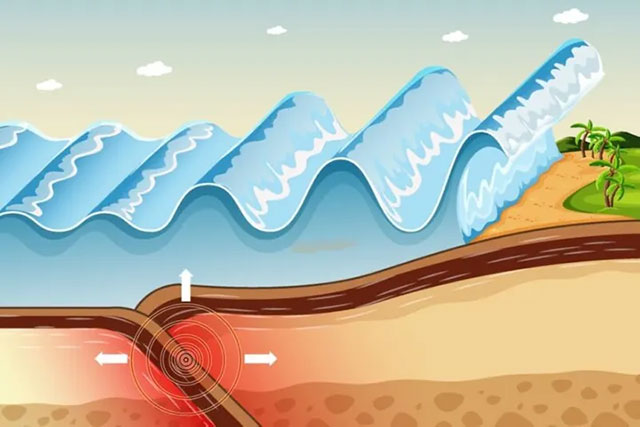
\includegraphics[width=4cm]{Hinh/CT66}}
\choiceTF[t]
{\True Tốc độ truyền sóng thần tính được là $800\ km/h$}
{\True Biên độ lớn của sóng thần là nguyên nhân gây ra sức tàn phá nghiêm trọng}
{\True Tốc độ truyền sóng lớn khiến công tác cảnh báo gặp khó khăn}
{Bước sóng của sóng thần là $800\ m$}
\loigiai{
\begin{itemchoice}
\itemch Áp dụng $v = \dfrac{\lambda}{T} = \dfrac{800}{1} = 800\ km/h$
\itemch Biên độ càng lớn thì sóng càng mang nhiều năng lượng, gây phá hủy mạnh
\itemch Vận tốc lớn nên sóng đến bờ nhanh, khó cảnh báo kịp
\itemch Bước sóng là $800\ km$, không phải $800\ m$
\end{itemchoice}
}
\end{ex}
\begin{ex}
Một sóng cơ hình sin truyền theo trục $Ox$ có tốc độ truyền sóng v, bước sóng $\lambda$ và tần số f.
\choiceTF[t]
{Công thức liên hệ giữa tốc độ truyền sóng v, bước sóng $\lambda$ và tần số f của sóng là $\lambda= v.f$}
{Quãng đường mà sóng truyền đi được trong khoảng thời gian $\dfrac{1}{3f}$ là $3 \lambda$}
{\True Sóng cơ truyền từ môi trường này sang môi trường khác thì tần số không thay đổi}
{\True Giả sử sóng cơ truyền với tần số $10 ~Hz$, sau khoảng thời gian 2 phút thì quãng đường sóng truyền bằng 1200 lần bước sóng}
\loigiai{
\begin{itemchoice}
\itemch $\lambda=\dfrac{v}{f}$.
\itemch quãng đường mà sóng truyền đi được trong khoảng thời gian $\dfrac{1}{3 f}$ là $s=v. t=v \dfrac{1}{3. f}=\dfrac{\lambda}{3}$
\itemch
\itemch $s=v. t=v.120=\lambda. f.120=1200. \lambda$
\end{itemchoice}
}
\end{ex} \haidong{20}
\begin{ex}
Cá heo có thể phát ra sóng âm có tần số khoảng $250 \ kHz$ để giao tiếp với nhau và định vị các vật cản, con mồi.
\begin{center}

\includegraphics[width=10 cm]{images/105885}
\end{center}
\choiceTF[t]
{\True Sóng âm do cá heo phát ra là sóng siêu âm}
{Con người có thể nghe được sóng siêu âm}
{\True Lấy tốc độ sóng âm truyền trong nước là $1500$ mét mỗi giây. Bước sóng của sóng âm do cá heo phát ra là $0,6\ cm$}
{Có một dãy đá ngầm lớn trước hướng bơi của cá heo. Thời gian khi nó phát và nhận lại tín hiệu sóng là $5\ s$, giả sử cá heo đang bơi với tốc độ $72 \ km/h$. Khoảng cách từ cá heo tới dãy đá ngầm ngay khi nhận lại tín hiệu sóng là $3,8\ km$}
\loigiai{
\begin{itemchoice}
\itemch Sóng siêu âm là sóng âm có tần số lớn hơn $20 \, \text{kHz}$. Tần số sóng âm cá heo phát ra là $250 \, \text{kHz} > 20 \, \text{kHz}$ nên đây là sóng siêu âm.
\itemch Tai người có thể nghe được âm thanh trong dải tần từ khoảng $20 \, \text{Hz}$ đến $20 \, \text{kHz}$. Sóng siêu âm có tần số cao hơn $20 \, \text{kHz}$ nên con người không nghe được.
\itemch Bước sóng $\lambda = \dfrac{v}{f} = \dfrac{1500}{250 \times 10^3} = 6 \times 10^{-3} \, \text{m} = 0,6 \, \text{cm}$.
\itemch Thời gian sóng âm đi và về là $5 \, \text{s}$, vậy thời gian sóng âm đi đến đá ngầm là $t = \dfrac{5}{2} = 2,5 \, \text{s}$. Khoảng cách ban đầu từ cá heo đến đá ngầm là $d_0 = v.t = 1500 \times 2,5 = 3750 \, \text{m} = 3,75 \, \text{km}$.
Tốc độ cá heo là $72 \, \text{km/h} = 20 \, \text{m/s}$. Trong thời gian $5 \, \text{s}$, cá heo bơi được quãng đường $s = v_{caheo} \times 5 = 20 \times 5 = 100 \, \text{m} = 0,1 \, \text{km}$.
Khoảng cách từ cá heo tới dãy đá ngầm ngay khi nhận lại tín hiệu sóng là $d = d_0 + s = 3,75 + 0,1 = 3,85 \, \text{km}$.
\end{itemchoice}
}
\end{ex}
\begin{ex}
\immini[thm]{Trong giờ học thể dục, một bạn học sinh gắn một đầu dây rất dài có tính đàn hồi và không dãn vào một bức tường cố định, sau đó kích thích để đầu dây còn lại dao động bằng cách tay của bạn ấy kéo dây lên rồi hạ dây xuống theo phương thẳng đứng đều đặn như hình bên.}{

\includegraphics[width=6 cm]{images/2025_04_24_e31eca986abbba218779g-6}}
\choiceTF[t]
{\True Chắc chắn bạn đó đã tạo ra một sóng cơ truyền trên sợi dây}
{Trong trường hợp trên, nếu có sóng truyền trên sợi dây thì sóng đó thuộc loại sóng dọc}
{Nếu đầu dây được kích thích dao động bằng một nguồn dao động điều hòa với tần số là 2 Hz, thì chu kì của sóng truyền trên dây là 2 s}
{Nếu điểm cách đầu dây $0,8\ m$ bắt đầu dao động sau thời gian một giây kể từ lúc kích thích cho đầu dây dao động thì tốc độ truyền sóng truyền trên dây có giá trị là $0,8\ cm/s$}
\loigiai{ }
\end{ex}
\setcounter{ex}{0}
\PhanIII
\begin{ex}
Một sóng cơ truyền với tần số $10 ~Hz$, sau khoảng thời gian 1 phút thì quãng đường sóng truyền bằng bao nhiêu lần bước sóng?
\shortans[oly]{600} 
\loigiai{
\begin{itemize}
\item Trong 1 phút thực hiện được $N=\Delta t. f=60.10=600$ chu kì
\item Mỗi chu kì sóng truyền được một bước sóng, vậy trong thời gian 600 chu kì quãng đường truyền được 600 bước sóng
\end{itemize}
}
\end{ex} \haidong{20}
\begin{ex}
Một sóng mặt nước lan truyền với tốc độ $10 ~m/s$, khoảng cách 12 đỉnh sóng liên tiếp là $11 ~m$. Tần số sóng bằng bao nhiêu héc?
\shortans[oly]{10}
\loigiai{
Giữa 12 đỉnh sóng liên tiếp có 11 khoảng, khoảng cách 2 đỉnh sóng liên tiếp bằng một bước sóng
$\Rightarrow 11 \lambda=11 \Rightarrow \lambda=1 \Rightarrow f=\dfrac{v}{\lambda}=\dfrac{10}{1}=10~Hz$
}
\end{ex} \haidong{20}
\begin{ex}
Người ta gây ra một dao động với tần số $20 ~Hz$ ở đầu $O$ của một sợi dây rất dài, tạo nên sóng ngang hình sin lan truyền trên dây, sau $6 ~s$ sóng truyền được quãng đường $9,3 ~m$. Sóng truyền trên dây có bước sóng bằng bao nhiêu cm?\\ \shortans[oly]{7,75}
\loigiai{
7,75
}
\end{ex} \haidong{20}

\begin{ex}
\nguon{SGK - CTST} Một bạn học sinh đang câu cá trên hồ nước. Khi có sóng đi qua, bạn quan sát thấy phao câu cá nhô lên cao 6 lần trong $4 ~s$. Biết tốc độ truyền sóng là $0,5 ~m/s$. Khoảng cách giữa hai đỉnh sóng liên tiếp là bao nhiêu mét?
\shortans[oly]{0,4}
\loigiai{
\begin{itemize}
\item Phao câu cá nhô lên cao 6 lần trong $4 ~s$ tương ứng với $5 T=4 ~s$  suy ra $T=0,8 ~s$
\item Khoảng cách giữa hai đỉnh sóng liên tiếp là $\lambda=v . T=0,5 . 0,8=0,4 ~m$
\end{itemize}
}
\end{ex} \haidong{20}
\begin{ex}%[3P2KB-2][Loai1]
Cho biết tốc độ âm trong không khí là 300 m/s, lấy $g = 10\ m/s^2$. Độ sâu của giếng là 11,25 m. Bỏ qua mọi lực cản. Một người thả một viên đá từ miệng giếng đến đáy giếng cạn thì sau bao nhiêu giây sẽ nghe thấy tiếng động do viên đá chạm đáy giếng (làm tròn kết quả đến chữ số hàng phần trăm)? 
\shortans[oly]{1,54}
\loigiai{
\begin{itemize}
\item Giai đoạn 1: Hòn đá rơi tự do.
\item Giai đoạn 2: Hòn đá chạm vào đáy giếng phát ra âm thanh truyền đến tai người.\\
$\begin{cases}
\text{Thời gian vật rơi: } h=\dfrac{gt_1^2}{2}\Rightarrow t_1=\sqrt{\dfrac{2h}{g}}=\sqrt{\dfrac{2.11,25}{10}}=1,5\ s.\\
\text{Thời gian âm truyền từ đáy đến tai người: } t_2=\dfrac{h}{v}=\dfrac{11,25}{300}=0,0375\ s.\\
\end{cases}$
$\Rightarrow t_1+t_2=1,5375\ s.$
\end{itemize}
}
\end{ex} \haidong{20}
\begin{ex}
Cho một nguồn âm phát sóng âm có công suất không đổi trong một môi trường truyền âm đẳng hướng và không hấp thụ âm. Một người đứng cách nguồn âm một đoạn $r\ (m)$ thì đo được cường độ sóng âm là I. Khi nguời rời xa nguồn thêm một đoạn $30 ~m$ thì cuờng độ sóng âm giảm đi 4 lần. Khoảng cách r ban đầu là bao nhiêu mét?
\\\shortans[oly]{30}
\loigiai{
30
}
\end{ex} \haidong{20}

